\newpage
\section{Настройка прав и ролей пользователей }

Для обеспечения работы пользователей в системе необходимо настроить для них права доступа к определенным разделам ФТМИС на выполнение определенных операций. Система разграничения доступа в ФТМИС базируется на основе понятия ролей (профилей прав) пользователей.

В системе имеется список доступных полномочий (прав пользователей). Его можно вызвать из меню \mm{Настройки \str Права пользователей} (Рисунок \ref{img_acs_priv}). Код и назначение привилегий предопределяется разработчиками.

\begin{figure}[ht]\centering
 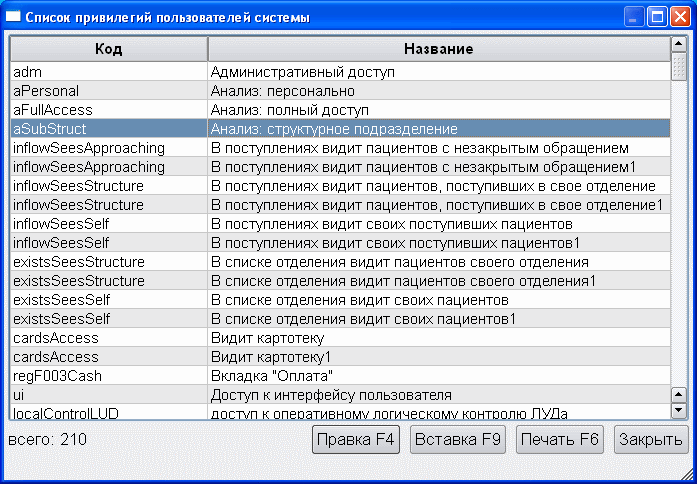
\includegraphics[width = 0.7\textwidth ,keepaspectratio]{acs_priv}
 \caption{Список привилегий пользователей}
 \label{img_acs_priv}
\end{figure}

Администратор системы должен создать для каждой группы пользователей набор привилегий. Такие наборы привилегии называются профилями прав или ролями пользователей. Они создаются из пункта меню \mm{Настройки \str Роли пользователей} (Рисунок \ref{img_acs_roles}).

Для добавления новой роли нужно нажать кнопку \btn{Вставка F9}, в открывшемся окне (Рисунок \ref{img_acs_role}) в поле \dm{Наименование} ввести название роли пользователя, отражающее ее суть (понятное для администратора системы), а в таблицу \dm{Разрешенные действия} добавить привилегии, необходимые для данной роли. Для добавления новой привилегии следует в нижней (пустой) строке дважды щелкнуть левой кнопкой мыши, активировав список привилегий, а затем выбрать нужную привилегию из списка. 

\begin{figure}[ht]\centering
 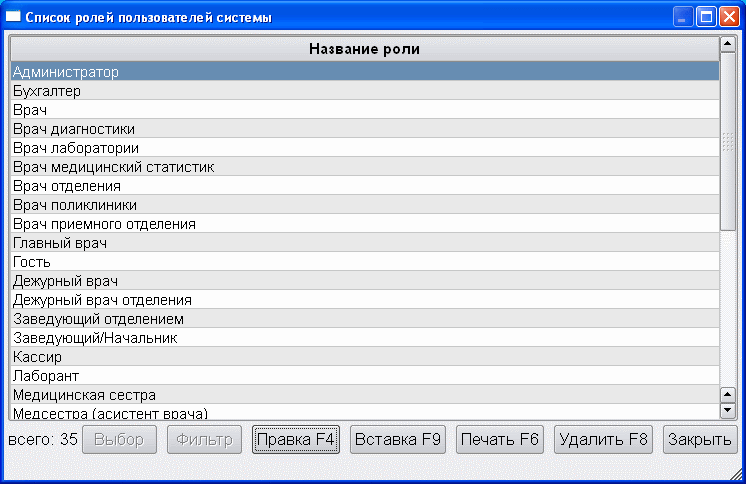
\includegraphics[width = 0.7\textwidth ,keepaspectratio]{acs_roles}
 \caption{Список ролей пользователей}
 \label{img_acs_roles}
\end{figure}

\begin{figure}[ht]\centering
 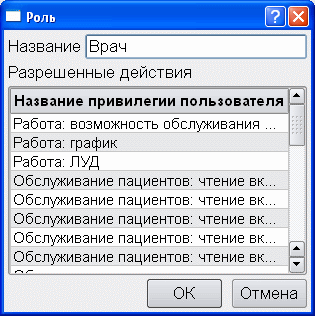
\includegraphics[width = 0.4\textwidth ,keepaspectratio]{acs_role}
 \caption{Настройка роли пользователя}
 \label{img_acs_role}
\end{figure}

Далее администратор может добавить пользователям созданную роль в справочнике \mm{Справочники \str Персонал \str Сотрудники}.

Для доступа к пункту меню \mm{Работа \str Обслуживание пациентов} у пользователя должна быть одна из следующих привилегий:
\begin{itemize}
 \item clientCardsAccess;
 \item clientRegRead;
 \item clientEventRead;
 \item clientInflowSeesSelf;
 \item clientInflowSeesStructure;
 \item clientInflowSeesApproaching;
 \item clientExistsSeesSelf;
 \item clientExistsSeesStructure.
\end{itemize}

Для работы с картотекой пациентов необходима привилегия <<cardsAccess>>, которая позволяет пользователю видеть картотеку пациентов.

Для работы с обращениями у пользователя должны быть некоторое из перечисленных в таблице \ref{tbl_acs_priv_obr} привилегий.

{\small
\begin{longtable}{|p{4cm}|p{5cm}|p{7.7cm}|}
\caption{Список привилегий для работы с обращениями \label{tbl_acs_priv_obr}} \\
\hline \rule{0pt}{15pt} \centering \textbf{Код права} & \centering \textbf{Название} & \hfil \textbf{Описание} \\ \hline
\endfirsthead
\hline \rule{0pt}{15pt} \centering \textbf{Код права} & \centering \textbf{Название} & \hfil \textbf{Описание} \\ \hline
\endhead
 clientEventCreate & 	Пациенты: обращения, создание &	Необходимо для создания новых обращений \\ \hline
 clientEventRead &	Пациенты: Обращения, чтение &	Делает доступным пункт меню \mm{Работа \str Обслуживание пациентов}, предоставляет возможность просмотра обращений \\ \hline
 clientEventUpdate &	Пациенты: обращения, изменение & 	Предоставляет возможность редактирования обращений \\ \hline
 changeExecPerson &	Имеет возможность изменять лечащего врача в обращении &	Так же пользователь может менять ответственного, если он создал это обращение \\ \hline
 changeFinanceSource & Имеет возможность изменять источники финансирования &	Для стационарных обращений \\ \hline
 evtDelAll & Имеет возможность удалять любое обращение &  \\ \hline 	
 evtDelOwn &	Имеет возможность удалять только свои обращения &	Свое обращение – это то, где пользователь является ответственным либо обращения, которые были созданы пользователем и не редактировались другими участниками системы \\ \hline
\end{longtable}
}

Для работы с действиями пользователю могут потребоваться следующие привилегии (Таблица \ref{tbl_acs_priv_act}):

\begin{table}[h]
\small
\topcaption{Привилегии для работы с действиями} \label{tbl_acs_priv_act} 
 \begin{tabular}{|p{3.8cm}|p{5cm}|p{7.9cm}|}
  \hline \rule{0pt}{15pt} \centering \textbf{Код права} & \centering \textbf{Название} & \hfil \textbf{Описание} \\ \hline
  copyPrevAction &	Копировать действия из предыдущих событий &	Делает доступной кнопку \btn{Копировать из предыдущего}  при редактировании действия \\ \hline
  loadActionTemplate &	Применять шаблоны действий &	Делает доступной кнопку  \btn{Загрузить шаблон}  при редактировании действия \\ \hline
 \end{tabular}
\end{table}

Для того чтобы пользователь имел возможность записи пациентов на прием, необходимо, чтобы у него была одна из следующих привилегий(Таблица \ref{tbl_acs_priv_reg}):

\begin{table}[h]
\small
\topcaption{Привилегии для записи на прием} \label{tbl_acs_priv_reg} 
 \begin{tabular}{|p{3.5cm}|p{5.9cm}|p{7.3cm}|}
  \hline \rule{0pt}{15pt} \centering \textbf{Код права} & \centering \textbf{Название} & \hfil \textbf{Описание} \\ \hline
  enquePrimary &	Может записывать как регистратор &	Запись по квотам <<Запись из регистратуры>> \\ \hline
  enqueOwn  &	Имеет возможность поставить в очередь как врач, записывающий пациента к себе на повторный прием &	Данная роль должна выдаваться врачам, ведущим амбулаторный прием. Запись по квотам <<Запись врачом на повторный прием>> \\ \hline
  enqueConsultancy	& Имеет возможность поставить в очередь как врач, записывающий пациента к другому врачу &	Запись по квотам <<Межкабинетная запись>> \\ \hline
 \end{tabular}
\end{table}

Для работы с листами назначений могут потребоваться некоторые из привилегий, приведенных в таблице \ref{tbl_acs_priv_ln}. \index{Листы назначений (настройки)}

{\small
\begin{longtable}{|p{4.2cm}|p{5cm}|p{7.5cm}|}
\caption{Привилегии для работы с листами назначений \label{tbl_acs_priv_ln}} \\
\hline \rule{0pt}{15pt} \centering \textbf{Код права} & \centering \textbf{Название} & \hfil \textbf{Описание} \\ \hline
\endfirsthead
\hline \rule{0pt}{15pt} \centering \textbf{Код права} & \centering \textbf{Название} & \hfil \textbf{Описание} \\ \hline
\endhead
clientPrescriptionsRead &	Имеет возможность просматривать и печатать лист назначений &	Возможность просмотра и печати листа назначений из карточки обращения \\ \hline
clientPrescriptions CreateOwn &	Имеет возможность создавать новые назначения только в тех обращениях, где пользователь является ответственным	& Делает доступной кнопку \btn{Создать назначение}  в листе назначений в карточках тех обращений, где текущий пользователь является ответственным  \\ \hline
clientPrescriptions CreateAll &	Имеет возможность создавать новые назначения во всех обращениях	& Делает доступной кнопку   \btn{Создать назначение}  в листе назначений в карточках всех обращений \\ \hline
clientPrescriptions EditOwn	& Имеет возможность редактировать, отменять назначения только в тех обращениях, где пользователь является ответственным	& Делает доступной для редактирования карточки ранее созданных назначений в листе назначений карточек обращений, где пользователь является ответственным  \\ \hline
clientPrescriptions EditAll	& Имеет возможность редактировать, отменять назначения во всех обращениях & 	Делает доступной для редактирования карточки ранее созданных назначений в листе назначений всех карточек обращений \\ \hline
wJobsOperating	& Имеет доступ к форме листа исполнений & Форма \dm{Лист назначений (исполнения)} является доступной для использования \\ \hline
clientPrescriptionsExec EditOwn	& Имеет возможность исполнять назначения только в рамках своего отделения  ЛПУ	& Форма \dm{Лист назначений (исполнения)} является доступной для использования, пользователь не имеет возможности изменения значения поля \dm{Подразделение}. В поле \dm{Подразделение} указано подразделение пользователя \\ \hline
clientPrescriptionsExec EditAll	& Имеет возможность исполнять назначения во всех отделениях ЛПУ	& Форма \dm{Лист назначений (исполнения)} является доступной для использования, имеется возможность выбора подразделения \\ \hline
clientPrescriptionsExec ChangeOrgStruct & Имеет возможность просматривать исполнения назначений в любом отделении ЛПУ в форме листа исполнений	& Форма \dm{Лист назначений (исполнения)} является доступной для просмотра исполнений и печати листа назначений, имеется возможность выбора подразделения \\ \hline
\end{longtable}
}

Рекомендуемые настройки прав пользователей по листам назначений приведены в таблице \ref{tbl_acs_roles_ln}.

{\small
\begin{longtable}{|p{7.6cm}|p{2.1cm}|p{2.1cm}|p{2.1cm}|p{2.1cm}|}
\caption{Рекомендуемые настройки прав пользователей \label{tbl_acs_roles_ln}} \\
\hline \rule{0pt}{15pt} \centering \textbf{Код права} & \centering \textbf{Врач отделения} & \centering \textbf{Дежур\-ный врач} & \centering \textbf{Медсест\-ра отделения} & \textbf{Админист\-ра\-ция ЛПУ} \\ \hline
\endfirsthead
\hline \rule{0pt}{15pt} \centering \textbf{Код права} & \centering \textbf{Врач отделения} & \centering \textbf{Дежур\-ный врач} & \centering \textbf{Медсест\-ра отделения} & \textbf{Адми\-нист\-ра\-ция ЛПУ} \\ \hline
\endhead			
clientPrescriptionsRead &	\centering $+$	&	\centering $+$		&	\centering $+$ & \hfil $+$ \\ \hline
clientPrescriptionsCreateOwn &		\centering $+$	& & & \\ \hline		
clientPrescriptionsCreateAll & &	\centering $+$ & & \\ \hline		
clientPrescriptionsEditOwn	&	\centering $+$ & & & \\ \hline			
clientPrescriptionsEditAll	&	&	\centering $+$ & & \\ \hline		
wJobsOperating	& &	 & 	\centering $+$	& \hfil $+$ \\ \hline
clientPrescriptionsExecEditOwn & & & \centering $+$ & \\ \hline	
clientPrescriptionsExecEditAll	& & & & \\ \hline			
clientPrescriptionsExecChangeOrgStruct	& & & & \hfil $+$ \\ \hline
\end{longtable}
}

\subsection{Настройка доступных типов действий для пользователей и ролей}

В системе существует возможность ограничить список типов действий, которые видит пользователь при создании очередной медицинской записи в карточке обращения, т.е. можно наложить фильтр на доступные типы действий. Возможна настройка ограничений для определенной роли или конкретного пользователя.

Для настройки фильтрации типов действий необходимо выбрать пункт меню \mm{Настройки \str Фильтр типов действий}. Откроется форма (Рисунок \ref{img_acs_tpact_filtr}) \dm{Фильтры типов действий}. В левой ее части находятся 2 вкладки. На вкладке \dm{Пользователи} настраиваются доступные типы действий для конкретных пользователей. На вкладке \dm{Роли} настраиваются доступные типы действий для всех пользователей, работающих под указанной ролью.

\begin{figure}[ht]\centering
 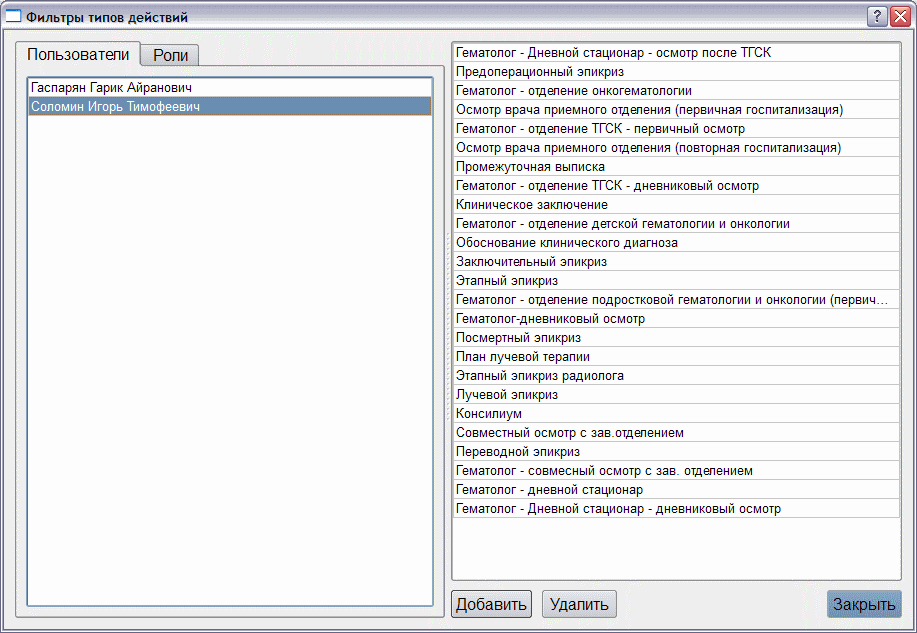
\includegraphics[width = 0.8\textwidth ,keepaspectratio]{acs_tpact_filtr}
 \caption{Форма настройки фильтраций типов действий для пользователей}
 \label{img_acs_tpact_filtr}
\end{figure}

\subsubsection{Создание нового правила фильтрации} \label{acs_tpactfiltr}

Для того чтобы создать новое правило фильтрации типов действий для пользователя или роли нужно перейти на соответствующую вкладку и нажать кнопку \btn{Добавить} в правом нижнем углу формы. Откроется новая форма \dm{Создание действий} (Рисунок \ref{img_acs_tpact_filtradd}). В левом верхнем углу, в поле со списком (второе сверху) в зависимости от вида создаваемого правила, следует выбрать фамилию пользователя или название роли. Далее, необходимо в таблицу \dm{Выбранные действия}, расположенную в правой части формы добавить типы действий, которые будут доступны указанному пользователю/роли. Добавление новых типов действий производится двойным щелчком мыши либо перетаскиванием (drag\&drop) соответствующего наименования типа действия из левой части формы в правую. В левой части может быть использовано как представление в виде списка, так и в виде дерева.

После того как список типов действий в таблице \dm{Выбранные действия} сформирован, необходимо нажать кнопку \btn{OK}  в правом нижнем углу формы. Текущая форма закроется, а в форме \dm{Фильтры типов действий} появится новая запись на активной вкладке.

\begin{figure}[ht]\centering
 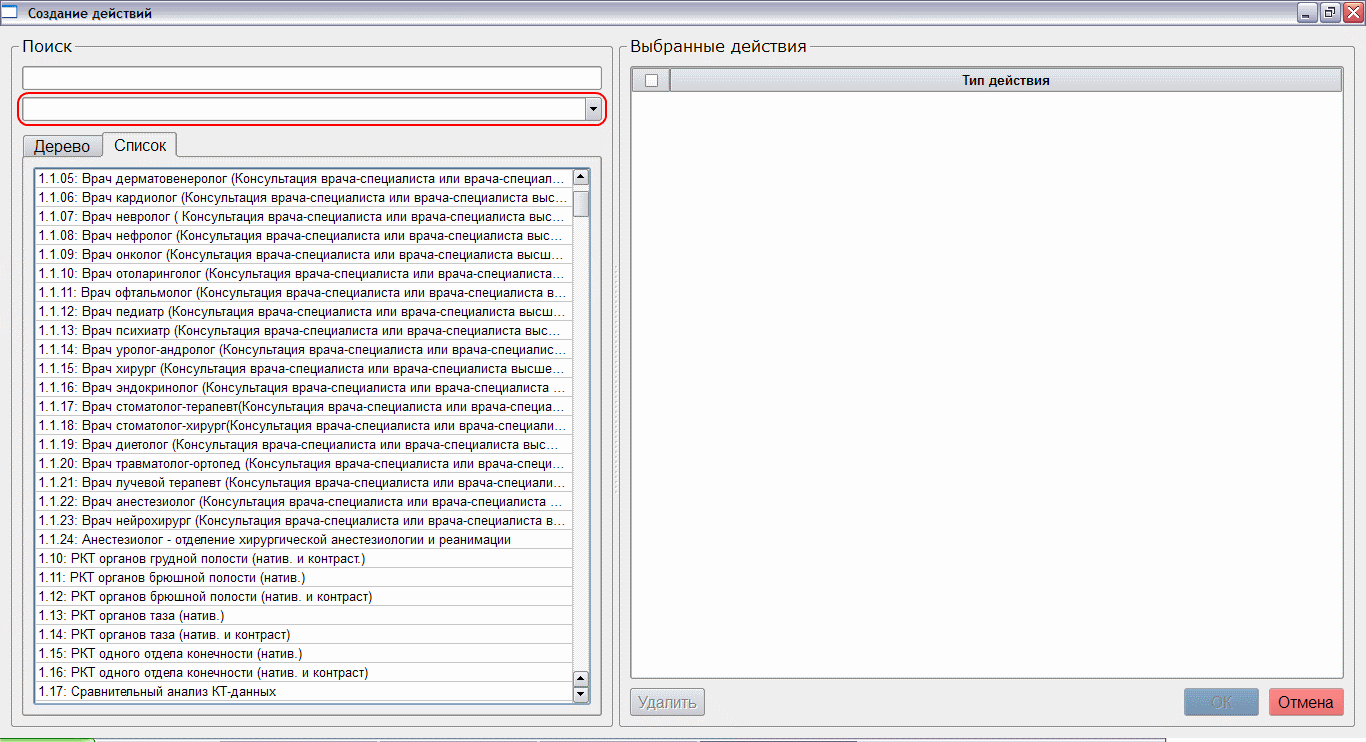
\includegraphics[width = 1\textwidth ,keepaspectratio]{acs_tpact_filtradd}
 \caption{Добавление правил фильтрации типов действий}
 \label{img_acs_tpact_filtradd}
\end{figure}

\subsubsection{Просмотр правила фильтрации}

Для того чтобы просмотреть список доступных типов действий для пользователя или роли, необходимо перейти на соответствующую вкладку (\dm{Пользователи} или \dm{Роли}) и установить курсор на определенной фамилии пользователя или названии роли, щелкнув по ней левой кнопкой мыши. После этого в правой части формы появится список доступных типов действий для выбранного пользователя/роли.

\subsubsection{Редактирование правил фильтрации}

Для редактирования списка доступных типов действий следует дважды щелкнуть левой кнопкой мыши по фамилии соответствующего пользователя или наименованию роли. Откроется форма \dm{Создание действий} (Рисунок \ref{img_acs_tpact_filtradd}), содержащее настройки фильтрации типов действий для выбранного пользователя/роли. Можно добавить или удалить типы действий из списка \dm{Выбранные действия}.

Добавление новых типов действий подробно описано в подразделе \ref{acs_tpactfiltr}

Для удаления наименования типа действия из списка следует установить напротив него флаг  \putx~ и нажать кнопку  \btn{Удалить} в правой нижней части формы. Для удаления наименований нескольких типов действий одновременно можно установить флажки   напротив их наименований, а затем нажать кнопку \btn{Удалить}.

После того как все изменения внесены в правило фильтрации следует нажать кнопку  \btn{OK} в правом нижнем углу формы. Будет осуществлен возврат к форме \dm{Фильтры типов действий}.

Для удаления правила фильтрации необходимо установить курсор на соответствующей фамилии пользователя или названии роли в левой части формы (Рисунок \ref{img_acs_tpact_filtr}) и нажать кнопку  \btn{Удалить} в правой нижней части формы.

\subsubsection{Порядок фильтрации типов действий}

При фильтрации типов действий установлен следующий порядок:
\begin{itemize}
 \item Если для текущего пользователя \textbf{не задано} правило фильтрации \textbf{по имени пользователя} и \textbf{не задано} правило фильтрации \textbf{по роли}, то при создании новой медицинской записи он может видеть \textbf{все типы действий}.
 \item Если для текущего пользователя \textbf{не задано} правило фильтрации \textbf{по имени пользователя}, но \textbf{задано} правило фильтрации \textbf{по роли}, то при создании новой медицинской записи он может видеть только  типы действий, определенные \textbf{для его роли}.
 \item Если для текущего пользователя \textbf{задано} правило фильтрации \textbf{по имени пользователя}, но \textbf{не задано} правило фильтрации \textbf{по роли}, то при создании новой медицинской записи он может видеть только типы действий, определенные \textbf{для данного пользователя}.
 \item Если для текущего пользователя \textbf{задано} правило фильтрации \textbf{по имени пользователя} и \textbf{задано} правило фильтрации \textbf{по роли}, то при создании новой медицинской записи он может видеть только типы действий, определенные \textbf{для данного пользователя}.
\end{itemize}
 
